% Página
\section{Confidencialidade com Criptografia Híbrida}

Na criptografia híbrida, Bob gera uma chave de dados aleatória (DEK) e usa uma cifra simétrica para proteger a mensagem. Em seguida, cifra a DEK com a chave pública de Alice. Neste exemplo, \(M1\) é a mensagem cifrada com AES-256-CBC e \(M2\) é a DEK cifrada com RSA-OAEP e SHA-256. Bob envia \(M1\), \(M2\) e o IV de \(M1\); Alice recupera a DEK com sua chave privada e então decifra \(M1\). O IV não é secreto, mas precisa acompanhar \(M1\). O servidor pode armazenar e encaminhar esses valores, mas não consegue recuperar a mensagem sem a chave privada de Alice.

Bob precisa obter a chave pública de Alice por um meio confiável e validar que ela realmente pertence a Alice, por exemplo conferindo um certificado ou um fingerprint por canal independente. Cifrar a DEK com RSA-OAEP protege essa chave para Alice, mas não autentica Bob.

\begin{figure}[H]
	\centering
	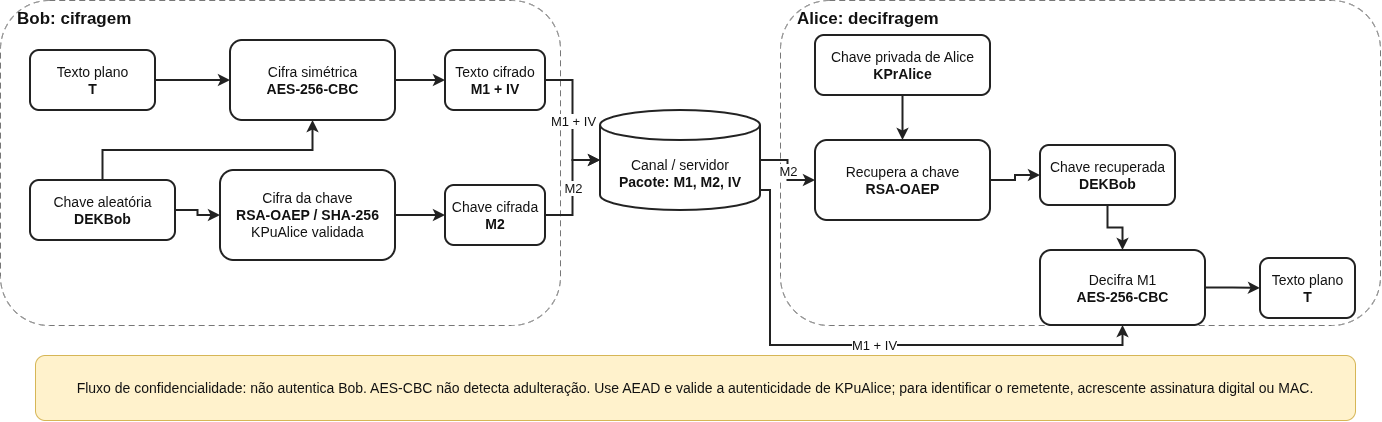
\includegraphics[width=\textwidth]{confidencialidade_autenticidade.png}
	\caption{Proteção híbrida da mensagem: AES cifra os dados e RSA-OAEP protege a chave de dados}
	\label{fig:confidencialidade_hibrida}
\end{figure}

\textbf{Criação do par de chaves de Alice}

Alice cria um par RSA. Ela mantém KPrAlice em segredo e disponibiliza KPuAlice com um mecanismo que permita a Bob autenticar a chave pública.
\begin{tcolorbox}[width=\textwidth]
	{\small
		\begin{verbatim}
		$ umask 077
		$ openssl genpkey -algorithm RSA -out KPrAlice.pem -pkeyopt rsa_keygen_bits:3072
		$ openssl pkey -in KPrAlice.pem -pubout -out KPuAlice.pem
		\end{verbatim}
	}
\end{tcolorbox}

\textbf{Cifragem híbrida (Bob)}

Bob gera uma DEK aleatória de 256 bits, cifra T.txt com AES-256-CBC e cifra a DEK com KPuAlice usando RSA-OAEP/SHA-256.
\begin{enumerate}
	\item Gerar a DEK e cifrar o texto. M1.iv deve acompanhar M1.enc.
	\begin{tcolorbox}[width=\textwidth]
	{\small
		\begin{verbatim}
		$ umask 077
		$ openssl rand -out DEKBob.bin 32
		$ DEK_HEX=$(od -An -v -tx1 DEKBob.bin | tr -d ' \n')
		$ IV_HEX=$(openssl rand -hex 16)
		$ printf '%s' "$IV_HEX" > M1.iv
		$ openssl enc -aes-256-cbc -K "$DEK_HEX" -iv "$IV_HEX" \
		  -in T.txt -out M1.enc
		\end{verbatim}
	}
	\end{tcolorbox}

	\item Cifrar a DEK com a chave pública autenticada de Alice, gerando M2.
	\begin{tcolorbox}[width=\textwidth]
	{\small
		\begin{verbatim}
		$ openssl pkeyutl -encrypt -in DEKBob.bin -inkey KPuAlice.pem -pubin \
		  -out M2.enc -pkeyopt rsa_padding_mode:oaep \
		  -pkeyopt rsa_oaep_md:sha256 -pkeyopt rsa_mgf1_md:sha256
		\end{verbatim}
	}
	\end{tcolorbox}

	\item Enviar M1.enc, M1.iv e M2.enc para Alice ou armazená-los no servidor para ela recuperar depois.
\end{enumerate}

\textbf{Decifragem (Alice)}

Alice usa KPrAlice para recuperar a DEK de M2 e, com essa DEK e o IV, decifra M1.
\begin{enumerate}
	\item Recuperar a DEK de M2.
	\begin{tcolorbox}[width=\textwidth]
	{\small
		\begin{verbatim}
		$ openssl pkeyutl -decrypt -in M2.enc -inkey KPrAlice.pem \
		  -out DEKBob.bin -pkeyopt rsa_padding_mode:oaep \
		  -pkeyopt rsa_oaep_md:sha256 -pkeyopt rsa_mgf1_md:sha256
		\end{verbatim}
	}
	\end{tcolorbox}

	\item Decifrar M1 com a DEK recuperada e o IV associado.
	\begin{tcolorbox}[width=\textwidth]
	{\small
		\begin{verbatim}
		$ DEK_HEX=$(od -An -v -tx1 DEKBob.bin | tr -d ' \n')
		$ openssl enc -d -aes-256-cbc -K "$DEK_HEX" -iv "$(cat M1.iv)" \
		  -in M1.enc -out T.txt
		\end{verbatim}
	}
	\end{tcolorbox}
\end{enumerate}

\textbf{Limites deste exemplo}

AES-CBC fornece confidencialidade, mas não integridade: alterações em \(M1\) ou no IV podem não ser detectadas e podem modificar o texto decifrado. O fluxo também não prova que Bob enviou a mensagem, e RSA-OAEP não autentica o remetente nem vincula o IV a \(M1\). Em produção, use um protocolo híbrido estabelecido que autentique o conteúdo e seus parâmetros, por exemplo com uma cifra AEAD como AES-GCM, garantindo um nonce único por chave; autentique Bob com uma assinatura digital verificada por uma chave pública confiável ou por um protocolo autenticado apropriado. A interface \texttt{openssl enc} usada neste exemplo não oferece cifras AEAD como AES-GCM, então não basta trocar o nome da cifra nos comandos. Os comandos com \texttt{openssl enc -K} são didáticos: a DEK aparece nos argumentos do processo e não deve ser manipulada dessa forma em produção.

\pagebreak

%Copyright
\vspace*{\fill}
\begin{flushright}
	\underline{\textit{Copyright}}\\
	All rights reserved to MT4 Tecnologia LTDA.\bigskip

	\underline{\textit{Autor}}\\
	Caio Abreu Ferreira [\href{mailto:cferreira@senhasegura.com}{cferreiras@senhasegura.com}] \bigskip\\
	
	\underline{\textit{MT4 Tecnologia Ltda.}}\\
	Rua Joaquim Antunes, 767 – Pinheiros – São Paulo\\
	Phone: +55 11 3065-7070\\
	\url{www.mt4.com.br}\\
	\href{mailto:support@senhasegura.com}{support@senhasegura.com}\\
\end{flushright}
